\section{Résultats et comparaison des méthodes}

\subsection{Résultats avec un jeu de données simple}

\subsubsection{Recherche à l'aide d'une heuristique}

\begin{figure}[!h]
    \centering
    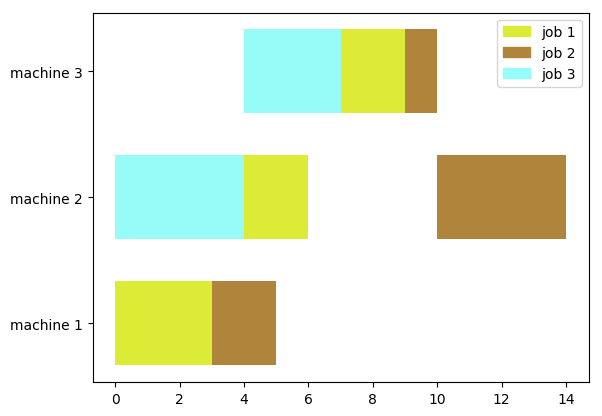
\includegraphics[]{results/test_shortest_operation.png}
\end{figure}

\frameboxbegin{Résultats}
Done in 14 units of time

Total time: 0.0033700000058161095 seconds 
\frameboxend

\newpage

\subsubsection{Recherche à l'aide de l'algorithme génétique}

\begin{figure}[!h]
    \centering
    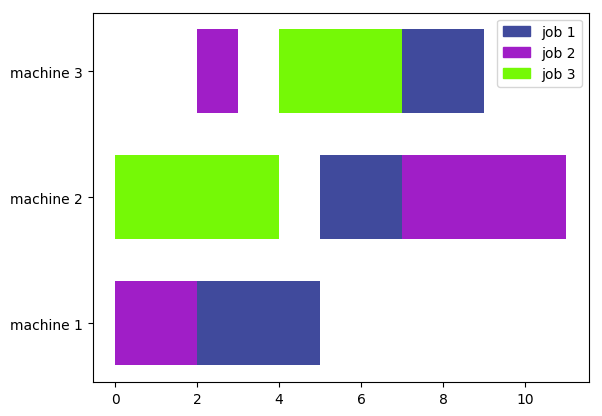
\includegraphics[]{results/test_genetic.png}
\end{figure}

\frameboxbegin{Résultats}
Population: 10, Max Generation: 100

Done in 11 units of time

Total time: 2.63803599998937 seconds
\frameboxend

\newpage

\subsection{Barnes - setb4c9}

\subsubsection{Recherche à l'aide d'une heuristique}

\begin{figure}[!h]
    \centering
    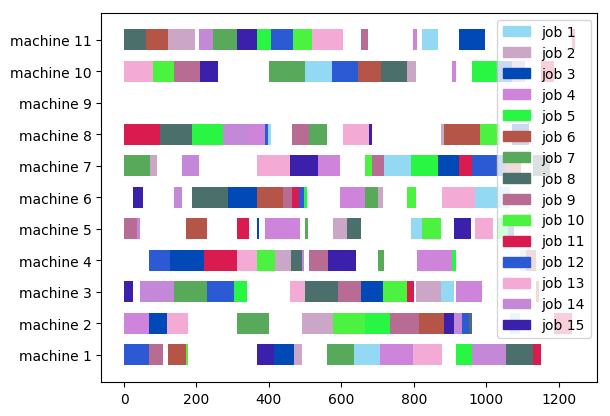
\includegraphics[]{results/barnes_setb4c9_shortest_operation.png}
\end{figure}

\frameboxbegin{Résultats}
Done in 1245 units of time

Total time: 0.04628799999773037 seconds 
\frameboxend

\newpage

\subsubsection{Recherche à l'aide de l'algorithme génétique}

\begin{figure}[!h]
    \centering
    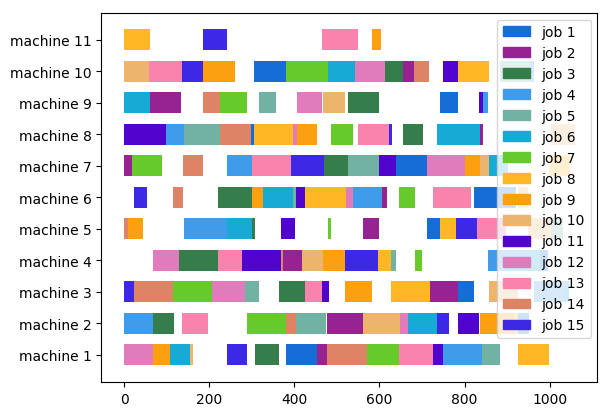
\includegraphics[]{results/barnes_setb4c9_genetic.png}
\end{figure}

\frameboxbegin{Résultats}
Population: 10, Max Generation: 300

Done in 1158 units of time

Total time: 17.04063700000006 seconds
\frameboxend